\subsection{MMU}
	Die Memory Management Unit wurde folgendermaßen implimentiert. Im linkerfile Skript werden die Startaddresse des INT RAM und des EXT DDR definiert. Es werden eine L1 und eine L2 Tabelle verwendet. Die virtuelle Addresse wird folgendermaßen auf eine physikalische Addresse gemappt:\\
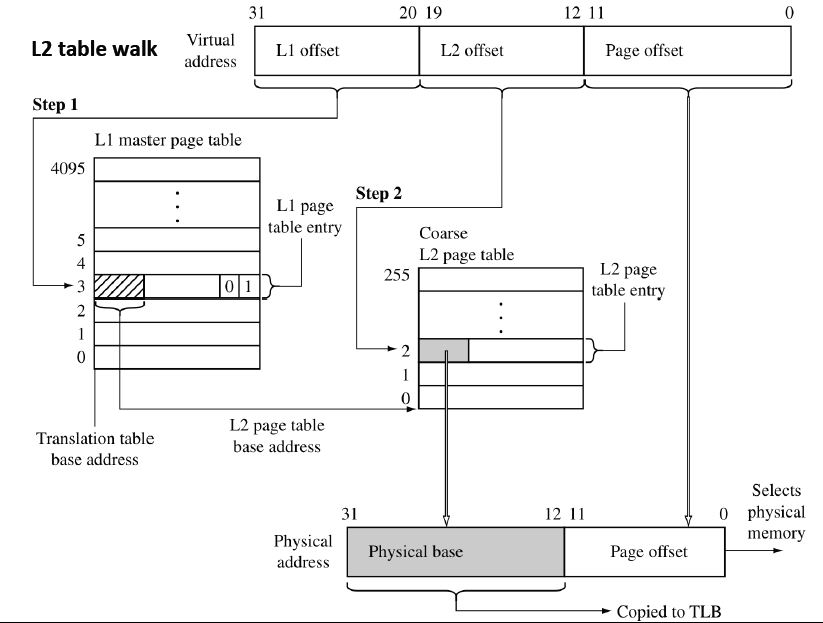
\includegraphics[scale=0.5]{images/VirtuellerSpeicher.png} 

Dabei werden die ersten 3 Hex-Zahlen für den Index in der L1 Tabelle verwendet.Der Inhalt der L1 Tabelle entspricht der Addresse der L2Tabelle. Die nächsten 2 Hex-Zahlen werden für den Index der L2 Tabelle verwendet. In Ihr steht die physikalische Addresse.\\
Für die L1 Tabelle wurden section pages verwendet (1MB) und für die L2 Tabelle wurden small pages (4kB) verwendet.
Interessanter Weise wurde nur 1 Domäne verwendet, deren AP Flags auf 11 gesetzt wurden. Das bedeutet das der man lesen und schreiben darf. Leider konnten wir nicht herausfinden warum andere AP Flags nicht funktionieren. Eigentlich sollten z.B AP Lags wie 01 den Zugriff einschränken und nur im Userprocess lesen dürfen, aber wir hatten keinen Zugriff mehr egal ob User oder Kernel Prozess.\\

Der Kernel wird 1:1 in den INT bzw.EXT DDR RAM gemappt. Die Userprocesse wurden in den EXT DDR gemappt.
\newpage
